% (c) 2020 Stefan Antonowicz
% Based off of tex found at https://github.com/ludus-leonis/nipajin
% This file is released under Creative Commons Attribution-NonCommercial-ShareAlike 4.0 International License.
% Please do not apply other licenses one-way.

\renewcommand{\yggAdvancement}{%
  \mychapter{Advancement}{advancement}
}

\renewcommand{\yggAdvancementText}{%

 \mysection{Experiences}{advancement-experiences}

  Advancing your adventurer (also known as "leveling") allows you to become more powerful.  To gain levels, you need Experiences (XP).  When you get a certain amount of XP, you go up a level.


  \mytable{X c c }{
    \thead{Level} & \thead{Min XP} & \thead{Coin Type} \\
  }{
    1 & 0 & Iron \\
    2 & 1,000 & Iron \\
    3 & 3,000 & Silver \\
    4 & 6,000 & Silver \\
    5 & 11,000 & Silver \\
    6 & 19,000 & Gold \\
    7 & 32,000 & Gold \\
    8 & 53,000 & Gold \\
    9 (max) & 87,000 & - \\    
}

There are 3 main ways to gain XP: Adventuring, Looting, and Carousing


\mysection{Adventuring}{advancement-adventuring}

Think about the Savage Sword of Conan.  He's out there killing pteranodons and slaying an average of 3 men with one blow, but those feats of strength are all encounters in a chapter of his greater adventures.  They fit nicely in a handful of comic books ("part 3 of 3 - Escape from the Necromancer's Lair)".  The Arbiter is there to help you narrate the chapters of \mybold{your} Adventure, just like R.E.H. did for Conan.

At the end of an Adventure, when you return to Civilization to eat and drink your fill, the Arbiter can award you XP.  It's completely up to her how much this is!  A good rule of thumb is if the Adventure would close a comic series or end a TV arc or finish a section of a novel, that's a good time to assign some XP (Thundarr breaks the werewolf curse; Conan escapes the Demons of the Summit; Fafhrd and the Grey Mouser return to Lankhmar with Ohmphal's fingertips, etc.)



\mysection{Looting and Spending}{advancement-looting-spending}

\flavor{
  There comes a time, thief, when the jewels cease to sparkle, when the gold loses its luster, when the Authority room becomes a prison, and all that is left is a father's love for his child. \Tilde{King Osric}
}

Treasure you loot on your adventures must be spent in order to convert it to XP.  Money you acquire and spend outside of an Adventure doesn't count (so if you pickpocket some rube or setup an opium trade or steal from the king it doesn't count, unless the chapter of your Adventure is entitled "Steal Shit from the King").  This is up to the Arbiter's discretion.

Levels 1 and 2 are the \mybold{Iron levels}.  You get 1xp for every iron piece you loot AND spend in Civilization.  These don't have to be Iron pieces per se -  if you were to loot and spend a single \AU, you would gain 100xp (but you would need to be in a larger civilization to spend it!)

Levels 3-5 are the \mybold{Silver levels}.  You get 1xp for every silver piece you loot AND spend in Civilization 

Levels 6+ are the gold levels.  You get 1xp for for every gold piece you loot AND spend in Civilization


Any coins you spend in Civilization are converted to XP on a 1-to-1 basis, including:

\mybullet {
  \item The amount of money you have to spend to take a Vacation (100\FE; 50\AG; or 25\AU)
  \item Any gear, narcotics, mounts, etc. you buy while in Civilization
  \item Any money you spend on Occultism, Chymistry, Miracles, Medicinals, Staff Magic, Sword Magic, or Inscription
  \item Any money you spend on a Carousing
}

Keep in mind the size of the Civilization you're in - you can't spend gold in Small hamlets!

You'll note that it gets harder and harder to get XP with money as you go up in level.  This is by design - legendary heroes aren't getting experience taking money from orc babies, but by doing epic shit i.e. writing chapters in their Adventure.  In time, the jewels cease to sparkle...


\end{multicols}   



\mysection{Carousing}{advancement-carousing}

If you've spent all the money you can, Carousing is a way to convert any extra coins you've got lying around into XP on a 1-for-1 basis. Say how much money you're going to burn and roll a d20 on the chart below.  You get a +1 for every 100 coins you spend (rounded down)

    \begin{center}
      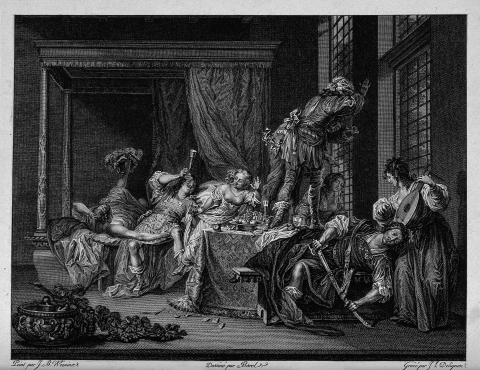
\includegraphics{Carousing}
    \end{center}


If you decide to go Carousing with a Pooka, you roll a d24 instead.  If a Pooka goes Carousing with you, \myital{they} get 10\% of any XP you make (this is in addition to your XP, they don't take from your XP).  They also have to roll a 20 on the table below, though.



\mytable{l X}{
  \thead{} & \thead{While Carousing you ...} \\
}{
  1  & Accidentally set the town aflame. Roll d6 twice. 1-2 burn down where you're staying; 3-4 some other house burns down; 5-6 a big chunk of town goes up in smoke. 1-2 no one knows it was you; 3-4 your fellow carousers know you did it; 5 someone else knows, perhaps a blackmailer; 6 everybody knows. \\
  2  &  Were robbed whilst unawares. Was it that saucy wench that you swear came to your room? You lose everything of value that you are carrying (Arbiter's discretion) \\
  3 & Talk shit and get called out. You get the XP for this Carousing, but you can't get any more until you do something really awesome designated by the Arbiter, like killing a legendary monster or stealing a legendary treasure. \\
  4 & Get in a fight, lose d3 teeth, get a black eye, or break your nose and you'll be sore (-d3 Grit, min 0) at the start of the next dungeon or fight. \\
  5 & Get alcohol poisoning. Roll a Save vs. Toxins. If you succeed, take 1 damage to Grit.  If you fail, take d6 damage to Grit \\
  6 & Are inducted into a cult. It takes your friends the rest of the Vacation to deprogram you.  Carousing earned you  -10\% XP \\
  7 &   Break some knuckles punching a dude. No two-handed weapons/shields until you Vacation again \\
  8 & Hangover from Hell. Roll twice on the Hang Over effect and take \mybold{both}  effects \\
  9 & Are mistaken for someone else, and charged with their tab. Pay 30\% more money (no xp for it) or wake up in the slammer. \\
  10  & Wake up in stocks. Authorities let you out after a day. \\
  11 & Gain reputation as a lecherous lush. Social interactions in this town are \myital{awkward.}  \\
 12 & Adapt to all the partying. You get +2 to your Save vs Toxins until the next Vacation \\
 13 &Gain 3 rumors about the next adventure  \\
  14  &Totally see through the Snail Knight's disguise, but are cool about it, and he will show up when you need him most. \\
  15 & Dice are hot. Get d100 coins  \\
  16 &Have an epic night and end up with a sweet scar.  \MAX Presence goes up \DCUP  \\
  17  & Win a bar bet and gain the services of two henchmen with low morale for a month. They may stay on if you pay them  \\
  18 & Run into a long-lost relative. Maybe they want to go adventuring with you?! (henchman - high morale)  \\
  19 &  Are mistaken for an important figure and the party gets really going. +25\% XP.  \\
  20+ & Have a lot of fun and get plenty of relaxation \\  
}

\example {
    Mad Tom, Aelfirth, and Stump Beefknob (a Pooka) are all level 1, returning from the Boudoir of Unutterable Horrors laden with loot.  They make their way to Arkham (a Small city, perfect for spending Iron) and elect to take a Vacation.  The Arbiter awards them all 500 xp right off the bat for surviving and killing the Thing Beneath the Bed (completing a Chapter in the Arbiter's story).  They each spend the 100\FE required to take a Vacation, and spend an additional 100\FE each on equipment (plus a trip to the Sanitarium for Mad Tom). They each have 400\FE left.  They all decide to go Carousing together and spend their remaining iron pieces.  

    Because they're Carousing with a Pooka, Mad Tom and Aelfirth both roll a d24 - Stump rolls a d20.  Tom rolls a 14 (10 + 4 for the 400\FE) and sees through the Snail Knight's disguise; now he has an ally that he notes on his character sheet.  Aelfirth rolls a 7 (3+4, bad luck!) and gets alcohol poisoning.  Stump rolls a 15 - looks like he won 43\FE gambling.  

    Tom and Aelfirth get 1,100 xp (500 from the Arbiter, 100 from the Vacation, 100 from equipment, and 400 from going Carousing).  Stump earns 1,180xp (500 from the Arbiter, 100 from the Vacation, 100 from the equipment, 400 from Carousing, plus an extra 10\% of the 800 Tom and Aelfirth collectively earned from their Carousing).
  }


  \begin{multicols*}{2}\raggedcolumns

  \mysection{Gaining a Level}{advancement-leveling}

  You made it to the next level!  Congratulations!

  \mynumlist {
    \item Regardless of your Trope or Species, roll your \FLESH twice and add the best result to your Grit.
    \item \mybold{Choose three} of the Virtues listed below
  }

\example{
  \mylist {
    \item \mybold{If you've just reached 2nd or 3rd level}, 

you can pick from the Any or Iron lists; 
    \item \mybold{If you've just reached 4, 5, or 6th level},

you can pick from the Any, Iron, or Silver lists; 
    \item \mybold{If you've just reached 7, 8, or 9th level},

you can pick from the Any, Iron, Silver, or Gold lists
  }
}



  If a Virtue doesn't have a Keyword next to it, you can take it as many times as you like every level.  Otherwise:

  \mylist {
    \item \mybold{Special} You can only get this Virtue one time per level
    \item \mybold{Unique}  You can only get this Virtue one time, ever
  }


    \begin{center}
  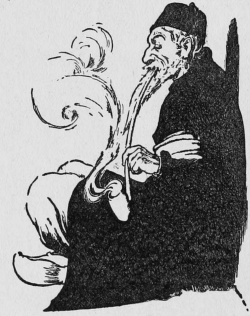
\includegraphics[scale=.75]{SeatedWizard}
  \end{center}

 \cbreak
 
  %%%%%%%%%%%%%%%%%%%%%%%%%%%%%%%%%%%%%%%%%%%%%%%%%%%%%%%%%%%%%%%%%%%%%%
  %%%%  ANY %%%%%%%%%%%%%%%%%%%%%%%%%%%%%%%%%%%%%%%%%%%%%%%%%%%%%%%
  %%%%%%%%%%%%%%%%%%%%%%%%%%%%%%%%%%%%%%%%%%%%%%%%%%%%%%%%%%%%%%%%%%%%%%  


  \mysubsection{Any Level}{advancement-leveling-any}

  \mybullet {
    \item Learn a new skill as if you were Trained in it (d8)
    \item Add 10 successes to any skill you know.  If the number of successes is enough to move your skill to the next level, it moves to the next level.
    \item Learn a new Dialect or Idiolect
    \item Move two different Saves to the next level (Defenseless to Preserved; Preserved to Protected; etc) 
    \item Move two different Stats (Tangible and/or Intangible) \DCUP.
    \item Learn two new languages of your choice
    \item Move your \DEATH to the next level (Precarious to Tough; Tough to Resilient; etc)
  }

  %%%%%%%%%%%%%%%%%%%%%%%%%%%%%%%%%%%%%%%%%%%%%%%%%%%%%%%%%%%%%%%%%%%%%%
  %%%%  IRON %%%%%%%%%%%%%%%%%%%%%%%%%%%%%%%%%%%%%%%%%%%%%%%%%%%%%%%
  %%%%%%%%%%%%%%%%%%%%%%%%%%%%%%%%%%%%%%%%%%%%%%%%%%%%%%%%%%%%%%%%%%%%%%    

  \mysubsection{Iron Levels}{advancement-leveling-iron}

  \myital{2nd and 3rd level}


  \myhighlight{Sellswords}{advancement-leveling-iron-sellswords}

  \mybullet {
    \item Move your Deed Die \DCUP \mybold{[Special]} 
    \item Upgrade your Armor one step (Light to Medium; Medium to Heavy) for no financial cost.
    \item Gain a normal weapon of your choice at no financial cost.
    \item Learn the Virtue \mylink{Blademaster}{sellsword-virtue-blademaster} \mybold{[Unique]} 
    \item Learn the Virtue \mylink{Lethal}{sellsword-virtue-lethal} \mybold{[Unique]} 
    \item Learn the Virtue \mylink{Three Kills Per Stroke}{sellsword-virtue-three-kills} \mybold{[Unique]} 
    \item \mybold{Danger Sense:} you (alone) cannot be Surprised (including the Drop) \mybold{[Unique]} 
    \item \mybold{Warding:} Choose an Ally at the start of Combat.  You must keep that Ally Close to you.   If that ally would take damage from a physical attack, you can choose to take the damage for them instead. \mybold{[Unique]} 
  }


  \myhighlight{Knaves}{advancement-leveling-iron-knaves}

  \mybullet {
    \item Move your Luck Die \DCUP \mybold{[Special]} 
    \item Upgrade your Armor one step (Light to Medium; Medium to Heavy) for no financial cost.
    \item Gain a normal weapon of your choice at no financial cost.
    \item Gain a new Whisper at Apprentice (d4) rank.
    \item Advance a Whisper from Apprentice to Footpad (d6) rank.
    \item Learn the Virtue \mylink{Deadeye}{knave-virtue-deadeye}.  Requires Whispers of the Bride \mybold{[Unique]} 
    \item Learn the Virtue \mylink{Mummy's Curse}{knave-virtue-mummys-curse}  \mybold{[Unique]} 
    \item \mybold{Slippery:} Once per Session, you can automatically escape from something that is restraining you and that you could plausibly escape from. This includes grapples, lynchings, and awkward social situations, but not sealed coffins.  \mybold{[Unique]} 
  }


  \myhighlight{Philosophers}{advancement-leveling-iron-philosophers}

  \mybullet {
    \item Learn the \mylink{The Crux of Blood}{philosopher-virtue-blood} \mybold{[Unique]} \\~ \\~  If you already know it, gain +1 Blood \POOL and write an additional spell inside your skull.  This must be a spell you have in your possession, either in a Grimoire or on a Fetish. \mybold{[Special]} 
    \item Learn \mylink{Wizardry}{philosopher-virtue-wizardry} (requires the Crux of Blood) \mybold{[Unique]}   
    \item Learn the \mylink{The Crux of Knowledge}{philosopher-virtue-knowledge} \mybold{[Unique]}. 
    \item If your Knowledge Die is a d10, you can increase it \DCUP (d12) \mybold{[Unique]}
    \item Learn \mylink{Leechcraft}{philosopher-virtue-leechcraft} (requires the Crux of Knowledge) \mybold{[Unique]} 
    \item Learn \mylink{Research: Chymistry}{philosopher-virtue-chymistry} \mybold{[Unique]} \\~ \\~ If you already have this Virtue, gain +1 Research \mybold{[Special]}
    \item Learn \mylink{Research: Inscription}{philosopher-virtue-inscription} \mybold{[Unique]}  \\~ \\~ If you already have this Virtue, gain +1 Research \mybold{[Special]}
    \item Learn \mylink{Research: Medicinals}{philosopher-virtue-medicinals} \mybold{[Unique]}  \\~ \\~ If you already have this Virtue, gain +1 Research \mybold{[Special]}
    \item Gain 3 Fetishes (d4 \UD) containing Wizardry arcana of your choice
  }




  \myhighlight{Mystics}{advancement-leveling-iron-mystics}

  \mybullet {
    \item Learn the \mylink{The Crux of Mojo}{mystic-virtue-mojo} \mybold{[Unique]} . \\~ \\~   If you already know it, move your Mojo \DCUP \mybold{[Special]} 
    \item Learn the \mylink{The Crux of Faith}{mystic-virtue-faith} \mybold{[Unique]} .\\~ \\~    If you already know it, gain +1 Faith \UD and move your \MAX Faith +2 \mybold{[Special]} 
    \item Learn the \mylink{The Gift of Grace}{mystic-virtue-grace} \mybold{[Unique]} . \\~ \\~   If you already know it, gain +1 Grace \UD \mybold{[Special]} 
    \item Learn \mylink{Cunning}{mystic-virtue-cunning} \mybold{[Unique]}.  \\~ \\~ If you already have this Virtue, gain +1 Cunning \mybold{[Special]}
    \item Learn \mylink{Aura}{mystic-virtue-armor}.  Requires the Crux of Mojo. \mybold{[Unique]} 
    \item Learn \mylink{Charms}{mystic-virtue-charms} \mybold{[Unique]} 
    \item Learn \mylink{Necromancy}{mystic-virtue-necromancy}. Requires the Crux of Mojo \mybold{[Unique]} 
    \item Learn the Liturgy of the Novitiates of your Authority or Small God.  The Liturgies of your Small God should be developed between you and the Arbiter \mybold{[Unique]} 
    \item If you know the Liturgy of the Novitiates of an Authority or Small God, you can learn that Authority or Small God's Liturgy of the Clerics \mybold{[Unique]} 
  }

  \myhighlight{Spriggan}{advancement-leveling-iron-spriggan}

  \mybullet {
    \item Gain +1 Remembrance \mybold{[Special]}
    \item Gain +1 Potential \mybold{[Special]}
    \item Gain +2 Sovereignty \mybold{[Special]}
    \item Gain a piece of magical material (a dragon's tooth, mithril ore, a ray of sunlight, etc) that could be used in Sword Magic.  Tell the Arbiter what this material is. \mybold{[Unique]}
    \item \mybold{Hyperawareness}.  Once per Session during Combat, you may become hyper-aware to the point of prescience.  \RS : Awareness at the top of the Moment.  If you succeed, you gain +8 to your Fight and Guard rolls for the remainder of the Moment. The effect ends at the end of Combat. \mybold{[Unique]}
    \item \mybold{Wisdom of the Forgotten}.  Once per Session, you can ask one of the Forgotten a question.  The Forgotten will answer you honestly, but possibly in a circuitous or cryptic fashion.  The question and answer are both limited to 3 words. \mybold{[Unique]}
  }

  \myhighlight{Murks}{advancement-leveling-iron-murks}

  \mybullet {
    \item Raise \mybold{all} of your Saves \DCUP \mybold{[Special]}
    \item Learn the Knave \mylink{Whisper of The Bride}{knave-whisper-the-bride} at the rank of Apprentice (d4). \mybold{[Unique]}
    \item Gain a piece of equipment from the Veins of the Earth sourcebook.
    \item Gain +4 Grit \mybold{[Special]}
    \item \mybold{Duelist}. You can use the Florentine Mighty Deed regardless of your \DEX \mybold{[Unique]}
    \item \mybold{Rock Whisperer}.  Not only will rocks speak with you, but you can convince them to move by speaking with them.  The rock(s) can't weigh more than 5kg collectively, can't be more than 10m away, and can't do things that rocks wouldn't be able to do (float on water, fly through the air without being thrown, etc); you can convince them to roll, "walk", or fall. \mybold{[Unique]}
  }



  \myhighlight{Pooka}{advancement-leveling-iron-pooka}

  \mybullet {
    \item Raise your Luck Die \DCUP \mybold{[Special]}
    \item Gain a suit of small-sized Light Armor.  If you already own a suit of small-sized Light Armor, gain a suit of small-sized Medium Armor.
    \item Learn the Knave \mylink{Whispers of Br'er Rabbit}{knave-whisper-brer-rabbit} at the rank of Apprentice (d4) \mybold{[Unique]}
    \item \mybold{Cold Turkey}: Remove all addictions and insanities you are currently afflicted by. \mybold{[Special]}
    \item \mybold{Must Be My Lucky Day!}: Once per \mylink{Session}{time-session}, you can do 1 of the following:  (a) win any Luck contest; (b) win any game of chance; (c) find extra narcotics just lying around (d2 \UD of any narcotic you want - if you don't use it before the next Session, it gets lost or evaporates or whatever); (d) regain 1 Flesh (enough to bring you off Death's Door) \mybold{[Unique]}
    \item \mybold{Calling in the Markers}: Roll your \LUCK, but don't move the die \DCDOWN if you roll a 1 or a 2.  You can purchase \SUM items from the Gear list, as long as the cost doesn't exceed \SUM x10 gold.  If you wish, you can distribute this gear immediately to the rest of your Band. \mybold{[Special]}
  }


  \myhighlight{Night Children}{advancement-leveling-iron-night-children}

  \mybullet {
    \item Raise you Looks die \DCUP \mybold{[Special]}

    \item Raise you Weird die \DCUP \mybold{[Special]}

    \item Raise you Gear die \DCUP \mybold{[Special]}

    \item Roll your Looks die and apply the result to your adventurer \mybold{[Special]}

    \item Roll your Weird die and apply the result to your adventurer \mybold{[Special]}

    \item Roll your Gear die and apply the result to your adventurer \mybold{[Special]}
  }


  %%%%%%%%%%%%%%%%%%%%%%%%%%%%%%%%%%%%%%%%%%%%%%%%%%%%%%%%%%%%%%%%%%%%%%
  %%%%  SILVER %%%%%%%%%%%%%%%%%%%%%%%%%%%%%%%%%%%%%%%%%%%%%%%%%%%%%%%
  %%%%%%%%%%%%%%%%%%%%%%%%%%%%%%%%%%%%%%%%%%%%%%%%%%%%%%%%%%%%%%%%%%%%%%  


  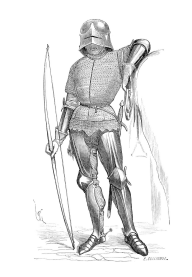
\includegraphics{Archer}

  \newpage


  \mysubsection{Silver Levels}{advancement-leveling-silver}

  \myital{4th, 5th, and 6th Level}

  \example {
    All Silver Virtues are Unique unless otherwise specified.
  }



  \myhighlight{Sellswords}{advancement-leveling-silver-sellswords}

  \mybullet{

    \item Gain d6+1 Grit (in addition to your \FLESH roll for gaining a level) \mybold{[Special]}

    \item Your \mylink{Unarmed attacks}{combat-damage-unarmed} do +1 damage. \mybold{[Special]}

    \item \mybold{Berserker}:  If you are \mylink{Dying}{combat-dying}, gain +8 to Fight and Guard rolls.  This bonus ends the moment you go above 0 Flesh.

    \item \mybold{Into the Wilds}: Once per Session, if you're in a wilderness setting, you can say that you know of a cache nearby hidden in a tree bole, under a cairn, etc.  The cache can contains one of: 1. d8 \UD of food and water; 2. a shortbow with d8 \UD of arrows; 3. a suit of normal sized Light Armor; 4. a war axe, spear, and set of 4 daggers; 5. a small minor item (lantern and a few flasks of oil, ok; vials of poison or a looking glass, not ok)

    \item \mybold{Rallying Cry}: Make an \RS : Presence at the top of the Moment. If you succeed, you can declare you are foregoing your Fight check to allow all Allies to win Init in the next Moment, and gain +2 to Fight and Guard rolls.  You can do this as many times in Combat as you like, but you must  \RS : Presence each time.

    \item \mybold{Sword Saint}:  Any weapon you use deals \DCUP damage.
  }


  \myhighlight{Knaves}{advancement-leveling-silver-knaves}

  \mybullet {
    \item Advance a single Whisper from Footpad to Sharper (d8).  Can be taken more than once. 
     
    \item \mybold{Unlabeled Package:} In a Medium or Large Civilization, you may spend any amount of money to buy an Unlabeled Package. When the package is unwrapped, you declare what it contains, provided (a) it didn't cost more than you originally paid, (b) is smaller than a 1m cube, (c) wouldn't take up more than 1 Significant Item slot (no storing 100,000au in an Unlabeled package, for example), (d) is mundane, and (e) would be available in the Civilization you came from 

    \item \mybold{Poisonous:} Once per \mylink{Vacation}{civilization-vacation}, you can create a d4 \UD Iron, Silver, or Gold Acid or Toxin.  You must still pay the monetary cost of the Acid or Toxin.    You no longer need to \RS : \DEX when handling Acids or Toxins. 

    \item \mybold{Brutal:} Requires Whispers of the Bride.  When attempting a Murder, you may use a \mylink{War Axe}{gear-weapons}, \mylink{Spear}{gear-weapons}, or \mylink{Mace}{gear-weapons} in addition to the other weapons allowed. You still must be Close to the Monster.  If you are using a War Axe and manage to slay the Monster, you may invoke the War Axe's \mylink{Cleave}{gear-weapon-cleave} ability to attack another Monster, but it doesn't count as a Murder, as you no longer have The Drop.

    \item \mybold{Silence is Golden:}  You no longer need to speak in order to perform your Whispers. 

    \item \mybold{Agile:}  Your \MD when wearing Light Armor is d20 

  }

  \myhighlight{Philosophers}{advancement-leveling-silver-philosophers}

  \mybullet {

      \item Once per Session, you can declare something to be true because you read it in a book. The base chance of the thing actually being true is 3 in 6. There has to be a plausible way you could know about it from reading books (new discoveries, minor details, and personal secrets are unlikely). You don't know whether or not it is true right away; the Arbiter will roll when it matters. You might only be partially correct, but you will never be catastrophically wrong. If you declare that bugbears fear albino goats, they will either fear albino goats or be indifferent to albino goats. They won't be driven into a murderous rage by them. If you have access to a library of 50 books, the base chance increases to 5 in 6

      \item If your Knowledge Die is a d12, you can increase it \DCUP (d16) \mybold{[Unique]}
    
      \item \mybold{Wisdom:} You have a reputation for wisdom.  If there's a weird problem, people will go to you first. If there's a mutiny and you aren't part of the cause, you will be spared.

      \item \mybold{Learned:}  Gain +1 Research \mybold{[Special]}

      \item \mybold{Surge:}  Once per Session, when rolling your Blood \POOL, you can make every die a natural 6

      \item \mybold{Knowledge is Power:}  You can cast spells off of Fetishes using your Knowledge \STATIC. 
  }

  \myhighlight{Mystics}{advancement-leveling-silver-mystics}

  \mybullet {
    \item If you know the Liturgy of the Clerics of an Authority or Small God, you can learn that Authority or Small God's Liturgy of the Apostles
    
    \item \mybold{Tongues of Fire:} You can initiate the willing into your faith by giving them 1 of your Faith die.  The Faith die must be placed inside of a Holy Symbol and given to the initiate. Free assent is required, but it can be compelled by other factors (like a dagger to the throat or other threats).  If the initiate is "willing", gain 2 Faith (the willingness of the initiate is at the discretion of the Arbiter). 
    
    \item \mybold{Limited Immunity:} Choose one source of damage from the following list: 1. iron stabbing weapons; 2. iron chopping weapons; 3. wooden bashing weapons; 4. non-magical fire; 5. drowning. You are completely immune to it. 
}
  

\begin{center}
  
\includegraphics{ManHat}
\end{center}



\mybullet {
    \item \mybold{Feyness:} you can detect magic, supernatural effects, and general weirdness. 30m range for minor enchantments, charms, and sorceries; 1km range for seriously worrying magical trouble. It might be a premonition, a vision, a cold shudder, a glowing aura, or just a sense that something is "wrong". You can see ghosts and spirits, and they will know and respect you (you never need to roll Sanity for seeing shades or horrors). You know if an item is magical by inspecting it for Minutes. 

    \item \mybold{Safe House:} Depending on the size of a Civilization you're in, you have a chance (Small: 25\%, Medium 75\%, Large 100\%) of finding other practioners of your faith - a coven, cult, church, or what-have-you.  Your brethren will give you information, food, and lodging for free - the amount of money you must pay to take a \mylink{Vacation}{civilization-vacation} reduced by half, but you still get the full XP as if you had spent the coin.  The Arbiter must share a rumor with you about your current or next adventuere - the clue might be obscure, but it must be true

    \item \mybold{Master of Puppets:}  Add +4 to your Necromancy rolls
  }


  \myhighlight{Spriggan}{advancement-leveling-silver-spriggan}

  \mybullet {
    \item Once per Session, you can touch as many iron weapons you wish and make them magical for 1 Minute.  Each weapon you touch will deal 1 Flesh damage to you.  The weapon will stay enchanted for Hours.  The weapon has no additional characteristics, but can hit Monsters only affected by Magic.

    \item \mybold{Dreams of Elfland:}  Once per Session, you can cause every living thing Close to you to fall into a magical slumber.  This works in all ways like the Wizardry spell Sleep. The victims get a Save vs. Hexes and the sleep lasts for d12 Markovian.  The Dreams of Elfland cannot differentiate between Allies and Monsters. 

    \item  \mybold{Anamnesis of the Elements:} you can use your Remembrance to summon and control Elemental creatures for Minutes. 

    \item  \mybold{Anamnesis of the Damned:} you can use your Remembrance to summon and control Demonic creatures for Moments.

  }

  \myhighlight{Murks}{advancement-leveling-silver-murks}

  \mybullet {
    \item Once per Session, you can step into a shadow and become \mylink{Invisible}{effect-invisible}.  You can use this to get the Drop on someone, but there must be a shadow present (you couldn't do this in the middle of a sunny field, for example). 

    \item Once per Session, you can speak to stones and have them reshape themselves.  The stones can't be bigger than 1m in any dimension.  The stone will reshape itself into anything you desire - a large rock could be shaped into a idol, a passage could be made through a wall (provided the wall was less than 1m thick).  The object created is rough hewn - fine detail isn't possible (Arbiter's discretion) 

    \item You can reach into a shadow and pull out a dagger. The dagger exists for as long as it is not exposed to sunlight.  The dagger is magical, and can have Toxins applied to it.  If the dagger takes a life it immediately dissapates.

    \item Advance \mylink{Whispers of the Bride}{knave-whisper-the-bride} from Apprentice to Footpad (d6) (requires Whispers of the Bride: Apprentice).
  }

    
  \myhighlight{Pooka}{advancement-leveling-silver-pooka}

  \mybullet {

    \item Advance \mylink{Whispers of Br'er Rabbit}{knave-whisper-brer-rabbit} from Apprentice to Footpad (d6) (requires Whispers of Br'er Rabbit: Apprentice). 

    \item \mybold{Rager:} Once per Session, you can host a Rager during a \mylink{Bivouac}{combat-resting}.  Every person who participates gets all of the benefits of taking a \mylink{Vacation}{civilization-vacation} (though they can't go Carousing or perform Research, Occultism, or Miracles). The next day everyone has make an \RS : \VIG. If they fail they are \mylink{Hung Over}{effect-hung-over}.

    \item \mybold{Wound Transference:}  You can transfer your Flesh to Allies on a 1-to-1 basis i.e. for every point of Flesh you transfer, you take 1 point of Flesh damage. You do not need to be touching the Ally, but you do need to be Close to them.  The wounds that appear on your body match the wounds taken by the Ally.  The point of Flesh transferred is enough to keep an Ally from Dying.

    \item \mybold{Fast Metabolism:} You are immune to Toxins, Curses, and Diseases of all sorts 
  }


  
  \myhighlight{Night Children}{advancement-leveling-silver-night-children}

  \mybullet {
    \item Add or subtract 1 to a Looks, Quirks, or Gear roll you just made  \mybold{[Special]} 
    \item Add or subtract 2 to a Looks, Quirks, or Gear roll you just made \mybold{[Special]} 
    \item Add or subtract 3 to a Looks, Quirks, or Gear roll you just made \mybold{[Special]}
    \item Add or subtract 4 to a Looks, Quirks, or Gear roll you just made \mybold{[Special]} 
  } 


  %%%%%%%%%%%%%%%%%%%%%%%%%%%%%%%%%%%%%%%%%%%%%%%%%%%%%%%%%%%%%%%%%%%%%%
  %%%%  GOLD %%%%%%%%%%%%%%%%%%%%%%%%%%%%%%%%%%%%%%%%%%%%%%%%%%%%%%%
  %%%%%%%%%%%%%%%%%%%%%%%%%%%%%%%%%%%%%%%%%%%%%%%%%%%%%%%%%%%%%%%%%%%%%%  


  \mysubsection{Gold Levels}{advancement-leveling-gold}

  \myital{7th, 8th, and 9th Level}

  \example {
    At Gold levels, you can learn \mybold{any} Iron level skill from any Trope (but not Species).  \\~ \\~ All Gold Virtues are Unique unless otherwise specified.
  }

  \myhighlight{Sellswords}{advancement-leveling-gold-sellswords}

  \mybullet {
    \item 4 men-at-arms pledge their blades to your cause. They are \mylink{Henchmen}{gear-henchmen} with Orderly morale; they expect nominal pay, room, and board - otherwise, they will need to make periodic Morale checks at the discretion of the Arbiter.  They have 6 Flesh and wear Light armor.  In Combat, these soldiers can each (a) grant you +1 to your Fight or Guard \RO; (b) grant +2 to damage; or (c) take any physical damage for you.  You have to specify what each man-at-arms is doing at the top of each Moment i.e. "2 are giving me +1 to Fight, 1 is giving me +2 damage, and I'm keeping one back to take damage in case things go south.  If a man-at-arms dies or leaves your service, they will be replaced with another when you take a \mylink{Vacation}{civilization-vacation}

    \item \mybold{Battle Rage:} Once per Session, if you are \mylink{Enraged}{effect-enraged}, you can use a Combat Action to kill every Monster in Close range provided they have 2 \HD or less.  If you do a good job describing this to the Arbiter, it will prompt a morale check in any Nearby Monsters if they have 4 \HD or less.

    \item \mybold{Righteous Blade:} Any weapon you use (including if you are fighting Unarmed) is considered Magical.

    \item \mybold{Surprise, Motherfucker!}  Markovian effects are immedialy reduced by \DCDOWN x2 for you (meaning a d8 Markovian effect will only be a d4, and a d4 will have no effect).

  }


  \myhighlight{Knaves}{advancement-leveling-gold-knaves}

  \mybullet {
    \item Advance a Whisper from Sharper to Master (d10) rank. Can be taken more than once. 
    
    \item \mybold{Surprise, Motherfucker!} Once per Adventure, at any time, you may declare that you are walking off-screen. During any Session of the Adventure, you may reveal yourself to have been a minor NPC in the background of the scene "all along" as long as there actually are minor NPCs in the background of the scene. You can always walk back on stage at any time, even climbing in a window. This ability is limited by plausibility.

    \item  \mybold{The Plan:} Once per Session, you can declare that you’ve been planning for this very situation all along. Everyone in the group gets +8 to any \RO attempts for Minutes.  You need to tell the Arbiter how you influenced prior actions to lead to this outcome.

    \item  \mybold{The Guild} You become the focal point of a new Thieves Guild.  3 \mylink{Henchmen}{gear-henchmen} with Orderly morale join your cause; they expect nominal pay, room, and board - otherwise, they will need to make periodic Morale checks at the discretion of the Arbiter. Outside of Combat, these thieves can each (a) grant you +1 to any \RO attempt; (b) grant you +1 to any \KNAVE attempt; (c) take any physical damage (like from a trap) for you.  The Knaves have 4 Flesh, 4 Grit, and wear no armor.  You can never have more than 3 Knaves in your employ at a time.
  }

  \myhighlight{Philosophers}{advancement-leveling-gold-philosophers}

  \mybullet {
      \item If your Knowledge Die is a d16, you can increase it \DCUP (d20) \mybold{[Unique]}
      \item Create your own Wizardry spell. Work out the details with the Arbiter. It'll cost you a minimum of 5,000 au.  Requires Wizardry.
      \item Create your own Leechcraft skill.  Work out the details with the Arbiter.  It'll cost you a minimum of 5,000 au.  Requires Leechcraft.
      \item \mybold{Apprentice}.  An apprentice joins you.  They are \mylink{Henchmen}{gear-henchmen} with Cowardly morale; they expect nominal pay, room, and board - otherwise, they will need to make periodic Morale checks at the discretion of the Arbiter.  They have 2 Flesh and wear no armor. The apprentice can (a) carry as many Grimoires or Fetishes as you wish without it taking any inventory space; (b) grant you +3 Research; (c) grant you +2 to your Leechcraft rolls; and (d) take any physical damage for you.  You can only have 1 apprentice at any time.
  }

  \myhighlight{Mystics}{advancement-leveling-gold-mystics}

  \mybullet {
    \item If you know the Liturgy of the Apostles of an Authority or Small God, you can learn that Authority or Small God's  Liturgy of the Saints

    \item \mybold{Fishers of Men:} Requires the Virtue \mylink{Crux of Faith}{mystic-virtue-faith}.  2 disciples of the Small God flock to your cause.  These disciples are \mylink{Henchmen}{gear-henchmen} who can provide 1 d4 Faith \POOL (like a Holy Symbol) and have Fanatic morale. If the disciples are Close to you, you may use their Faith as if it were your own; however, if a disciple's Faith is ever exhausted, they will leave your service in Days if it is not restored.  You can give a disciple one of your Faith \POOL at any time (subtracting it from your own), but they can never have more than 1 Faith.  During a \mylink{Vacation}{civilization-vacation}, you can ask your disciples to make a "Test of Faith", each rolling their Faith die.  If they roll a 4, another disciple joins your cause; if they Fail (roll a 1 or a 2), they lose their Faith Die.  You can immediately restore this Faith if you choose, but the disciples can only make 1 roll per Vacation.  You can never have more than 12 disciples.  

    \item \mybold{Charmed Circle:}  Requires the Virtue \mylink{Cunning}{mystic-virtue-cunning}.  A coven of 2 witches join their powers with yours.  These witches are \mylink{Henchmen}{gear-henchmen} who provide 1 Cunning and have Fanatic morale; additionally, they each grant you +1 on your Mojo rolls, provided they are Close to you. You can use their Cunning to practice Occultism during a \mylink{Vacation}{civilization-vacation}, but they must be "in sync" with you; synchronizing your Cunning with them takes a full Widdershins. 

During a \mylink{Vacation}{civilization-vacation} you can choose to "draw down the moon".  Each witch rolls their Cunning Die.  If they roll a 4, another witch joins the Coven; if they Fail (roll a 1 or a 2), the ritual consumes their magic - they don't die, but they can no longer provide any Cunning and will leave the coven at the first opportunity.  You can never have more than 12 other members in your coven.  

    \item  \mybold{Norn's Shears:}  You intercede on behalf of an Ally with Fate itself.  You can stop someone Close or Nearby from dying when there's no hope of survival, provided you can plausibly explain to the Arbiter how they survived ("she must have slipped and fallen out of the way of the dragon's breath at the last second" or "even though we saw him tumble down the Edge of the World, he must have grabbed onto a crevice").  You can only do this once, ever 
  }

\begin{center}
  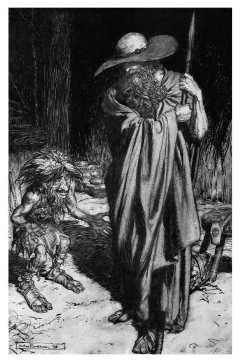
\includegraphics{Odin_1}
\end{center}



  \cbreak

  \myhighlight{Spriggan}{advancement-leveling-gold-spriggan}

  \mybullet {
    \item Choose one of the Forgotten whose True Name you know.  They are now bound to you permanently, as if they were a henchman or hireling. They will never be unsummoned or summoned by another, cost no Remembrance dice to keep or control, and are unswervingly loyal and treat you as a Small God.  When you reach level 9, you can choose to sacrifice them - through this haruspexy, you can divine the paths that will lead you back to Elfland (but will retire your character).

    \item You can learn the Virtue of Scrying, as detailed below.  Use your Awareness \UD to perform the Scrying.
  }

  \MYSTERY [
  Name= Scry,
  Link=spriggan-virtue-scry,
  Paradigm= Prophesy ,
  Save=  N ,
  Duration= Concentration ,
  Counter=  n/a  ,
  Keywords= None ,
  Target=   Something up to \SUM km away
]



This spell requires something to scry through - a mirror, a quiet pool, clouds, a bonfire, etc.  You create an invisible eye, ear, and mouth that can travel up to \SUM km away at a speed of 10km/hour.

\mylist {
  \item  For as long as you maintain concentration, everything the eye sees is reflected in the thing you're scrying through.  Other people can see what the eye sees if they're looking into the mirror, pool, clouds, bonfire, etc.  as well. The eye, being invisible, can see and be seen by invisible things.  

  \item The ear can hear for you as well.  You can use your Skill: Listen through the ear if you wish.

  \item You can speak through the mouth, including summoning the Forgotten to the location.

}

You can't separate the eye, ear, and mouth - they have to remain together.  The eye, ear, and mouth can fit through a space that you could reasonably pass the real thing through (a mouse hole, but not under a door)

\newpage

  \myhighlight{Murks}{advancement-leveling-gold-murks}

  \mybullet {
    \item Once per Session, you can travel through stone or earth up 10km away.  You need to have visited the destination and there must be uninterrupted stone or ground between yourself and the destination.  You can travel this distance in Minutes.   When you reach level 9,  you can use this ability to return to Svartalfheim if you choose (retiring your character)
    
    \item Advance \mylink{Whispers of the Bride}{knave-whisper-the-bride} from Footpad to Sharper (d8) (requires Whispers of the Bride: Footpad).    
  }

  \myhighlight{Pooka}{advancement-leveling-gold-pooka}

  \mybullet {
    \item \mybold{Martyrdom:}  If an Ally dies, you can take their place.  The Ally needs to be Close or Nearby to you, and they cannot have been dead for longer than Hours.  The body of the Ally must be in reasonably good shape - you can't save them if they've been reduced to ashes, for example.  You do not travel to the Isle of the Dead (being Unhallowed), but those who have been saved by Pooka are said to take on some of their "personality".
    
    \item Advance \mylink{Whispers of Br'er Rabbit}{knave-whisper-brer-rabbit} from Footpad to Sharper (d8) (requires Whispers of Br'er Rabbit: Footpad).
  }


  \myhighlight{Night Children}{advancement-leveling-gold-night-children}
  \mybullet {
    \item Choose a Looks, Weird, or Gear result as if you rolled the appropriate die.  For example, if your Gear die is a d8, you can choose any Gear result from 1 to 8.
    \item You can only be hurt by magical weapons, spells, and fire \mybold{[Unique]}
  }


  \example {
The Band of the Big Toe - Mad Tom (a Sellsword), Aelfirth (a Mystic), and Stump (a Pooka) - are all level 1, returning from their first adventure laden with loot. They make their way back to Lankhmar and elect to take a little Vacation. The Arbiter awards them all 500 xp right off the bat for surviving and killing the Thing Beneath the Stair (completing a Chapter in the Arbiter’s story). They each spend 100fe on their Vacation and an additional 100fe on equipment.  After selling a carpet and armoire they managed to secure, they each have 400fe left. They all decide to go Carousing together and spend their remaining iron pieces.

Because they’re Carousing with a Pooka, Mad Tom and Aelfirth both roll a d24 - Stump rolls a d20. Tom rolls a 14 (10 + 4 for the 400fe) and sees through the Snail Knight’s disguise; now he has an ally that he notes on his character sheet. Aelfirth rolls a 7 (3+4, bad luck!) and gets alcohol poisoning. Stump rolls a 15 - looks like he won 43fe gambling. Tom and Aelfirth get 1,100 xp (500 from the Arbiter, 100 from the Vacation, 100 from equipment, and 400 from going Carousing). Stump earns 1,180xp (500 from the Arbiter, 100 from the Vacation, 100 from the equipment, 400 from Carousing, plus an extra 10\% of the 800 Tom and Aelfirth collectively earned from their Carousing).

---

Time passes, and the Band gains more reknown.  Mad Tom reaches level 3; he has a Grit of 11.  He rolls his \FLESH (a d10) twice and takes the highest. He gets a 4 and a 7, so he now has 18 (11+7) Grit.  Tom now picks 3 new Virtues:  he opts to play it safe, moving his \VIG and Presence \DCUP; his Toxins and Hexes Saves \DCUP; and gaining a \DCUP on his Deed Die.  He may have instead wanted to take the Blademaster Virtue, or upgraded his Armor - but any way he breaks it down, he can only pick 3 new Virtues from the appropriate tables
  }

  \end{multicols*}
  \begin{multicols}{2}
}%
